\documentclass[11pt,a4paper]{article}

\usepackage[utf8]{inputenc}
\usepackage[T1]{fontenc}
\usepackage[english]{babel}
\usepackage{geometry}
\usepackage{booktabs}
\usepackage{enumitem}
\usepackage{graphicx}
\usepackage{xcolor}
\usepackage{hyperref}
\usepackage{fancyhdr}
\usepackage{titlesec}
\usepackage{tcolorbox}
\usepackage{siunitx}
\usepackage{caption}
\usepackage{float}
\usepackage{amsmath}
\usepackage{tikz}
\usetikzlibrary{arrows.meta, positioning}

\geometry{margin=2.5cm}

\definecolor{stepcolor}{RGB}{41, 128, 185}
\definecolor{warncolor}{RGB}{231, 76, 60}
\definecolor{tipcolor}{RGB}{39, 174, 96}
\definecolor{paramcolor}{RGB}{142, 68, 173}

\DeclareSIUnit\angstrom{\text {Å}}
\DeclareSIUnit{\revolution}{rev}
\DeclareSIUnit{\rpm}{\revolution\per\minute}
\DeclareSIUnit\mbar{mbar}
\newtcolorbox{warningbox}[1][]{colback=warncolor!5,colframe=warncolor!80,fonttitle=\bfseries,title={#1}}
\newtcolorbox{tipbox}[1][]{colback=tipcolor!5,colframe=tipcolor!80,fonttitle=\bfseries,title={#1}}
\newtcolorbox{parambox}[1][]{colback=paramcolor!5,colframe=paramcolor!80,fonttitle=\bfseries,title={#1}}

\pagestyle{fancy}
\fancyhf{}
\fancyhead[L]{\small Bilayer Lift-Off Protocol}
\fancyhead[R]{\small EGOFET Fabrication}
\fancyfoot[C]{\thepage}

\title{
    \vspace{-1cm}
    \textbf{PMGI SF5 / S1813 Bilayer Lift-Off Protocol} \\
    \large With DMSO Lift-Off for EGOFET Electrode Patterning
}
\author{
    e-MolMat Group -- ICMAB-CSIC \\
    \texttt{Protocol v1.0 -- \today}
}
\date{}

\begin{document}

\maketitle
\thispagestyle{fancy}

\begin{abstract}
This document describes an improved lift-off protocol for patterning
Cr/Au source--drain and gate electrodes on Kapton substrates. The method
replaces the standard single-layer Shipley S1813 process with a
\textbf{PMGI SF5 / S1813 bilayer} stack, combined with a
\textbf{DMSO-based lift-off} replacing the acetone/ultrasonic process.
The bilayer creates a controlled undercut profile during development that
prevents metal bridging on resist sidewalls, eliminating the need for
manual cotton-swab removal of residual gold from transistor channels.
\end{abstract}

\tableofcontents
\newpage

% ============================================================
\section{Introduction}
% ============================================================

\subsection{Problem Statement}

The current EGOFET fabrication protocol uses a single-layer Shipley S1813
positive photoresist for lift-off patterning of Cr/Au electrodes. This
produces vertical or slightly positive sidewall profiles, causing the
evaporated metal to form a continuous film on the resist sidewalls. During
lift-off, the acetone/ultrasonic baths cannot fully dissolve the resist
underneath this metal ``fence,'' leaving gold residue in the Source--Drain
channels. This residue must be removed manually with acetone-soaked cotton
swabs, which frequently damages the electrode pattern.

\begin{figure}[hbt!]
      \centering
      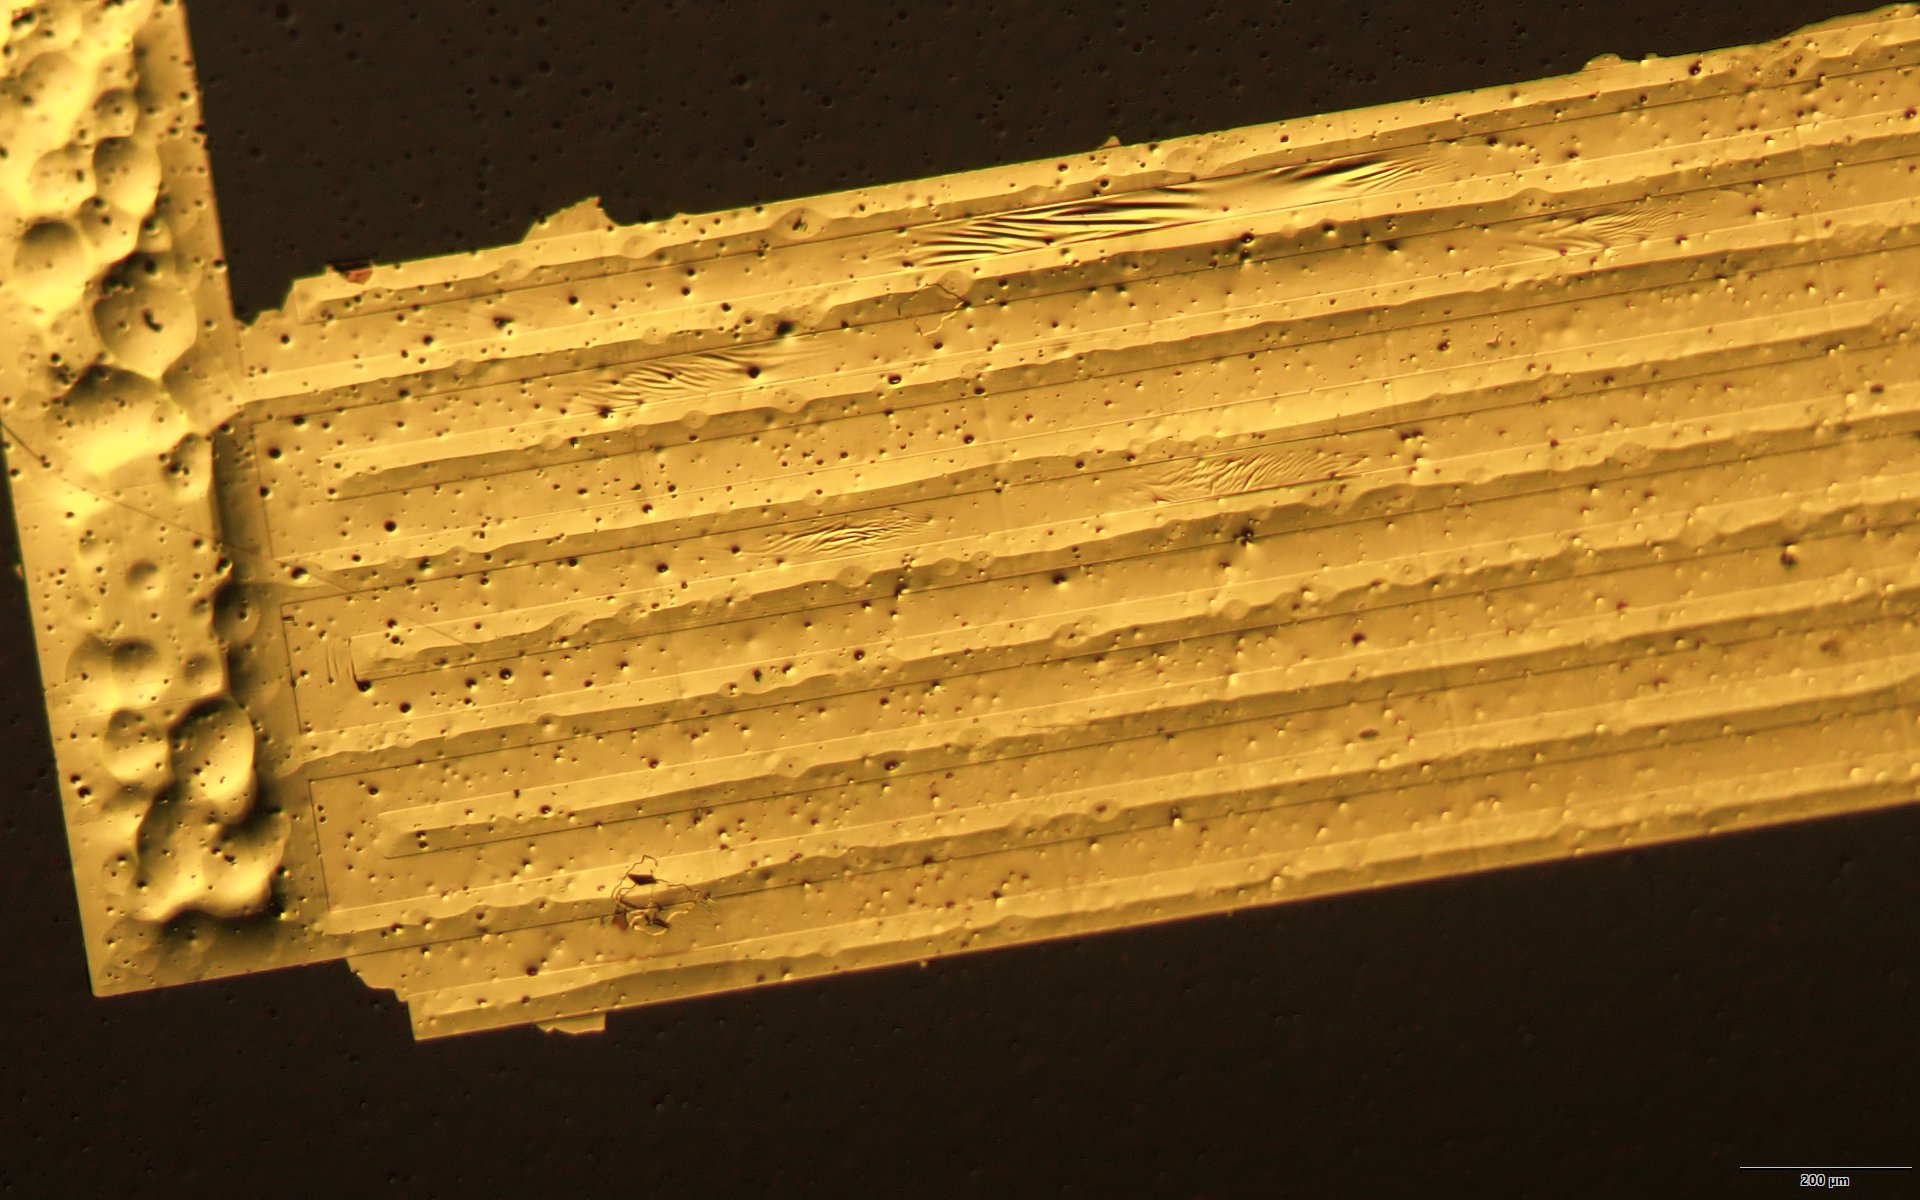
\includegraphics[width=0.4\textwidth]{../../data/photos/kapton/09072026_icn2/before/image_0708.jpg}\hspace{0.5cm}
      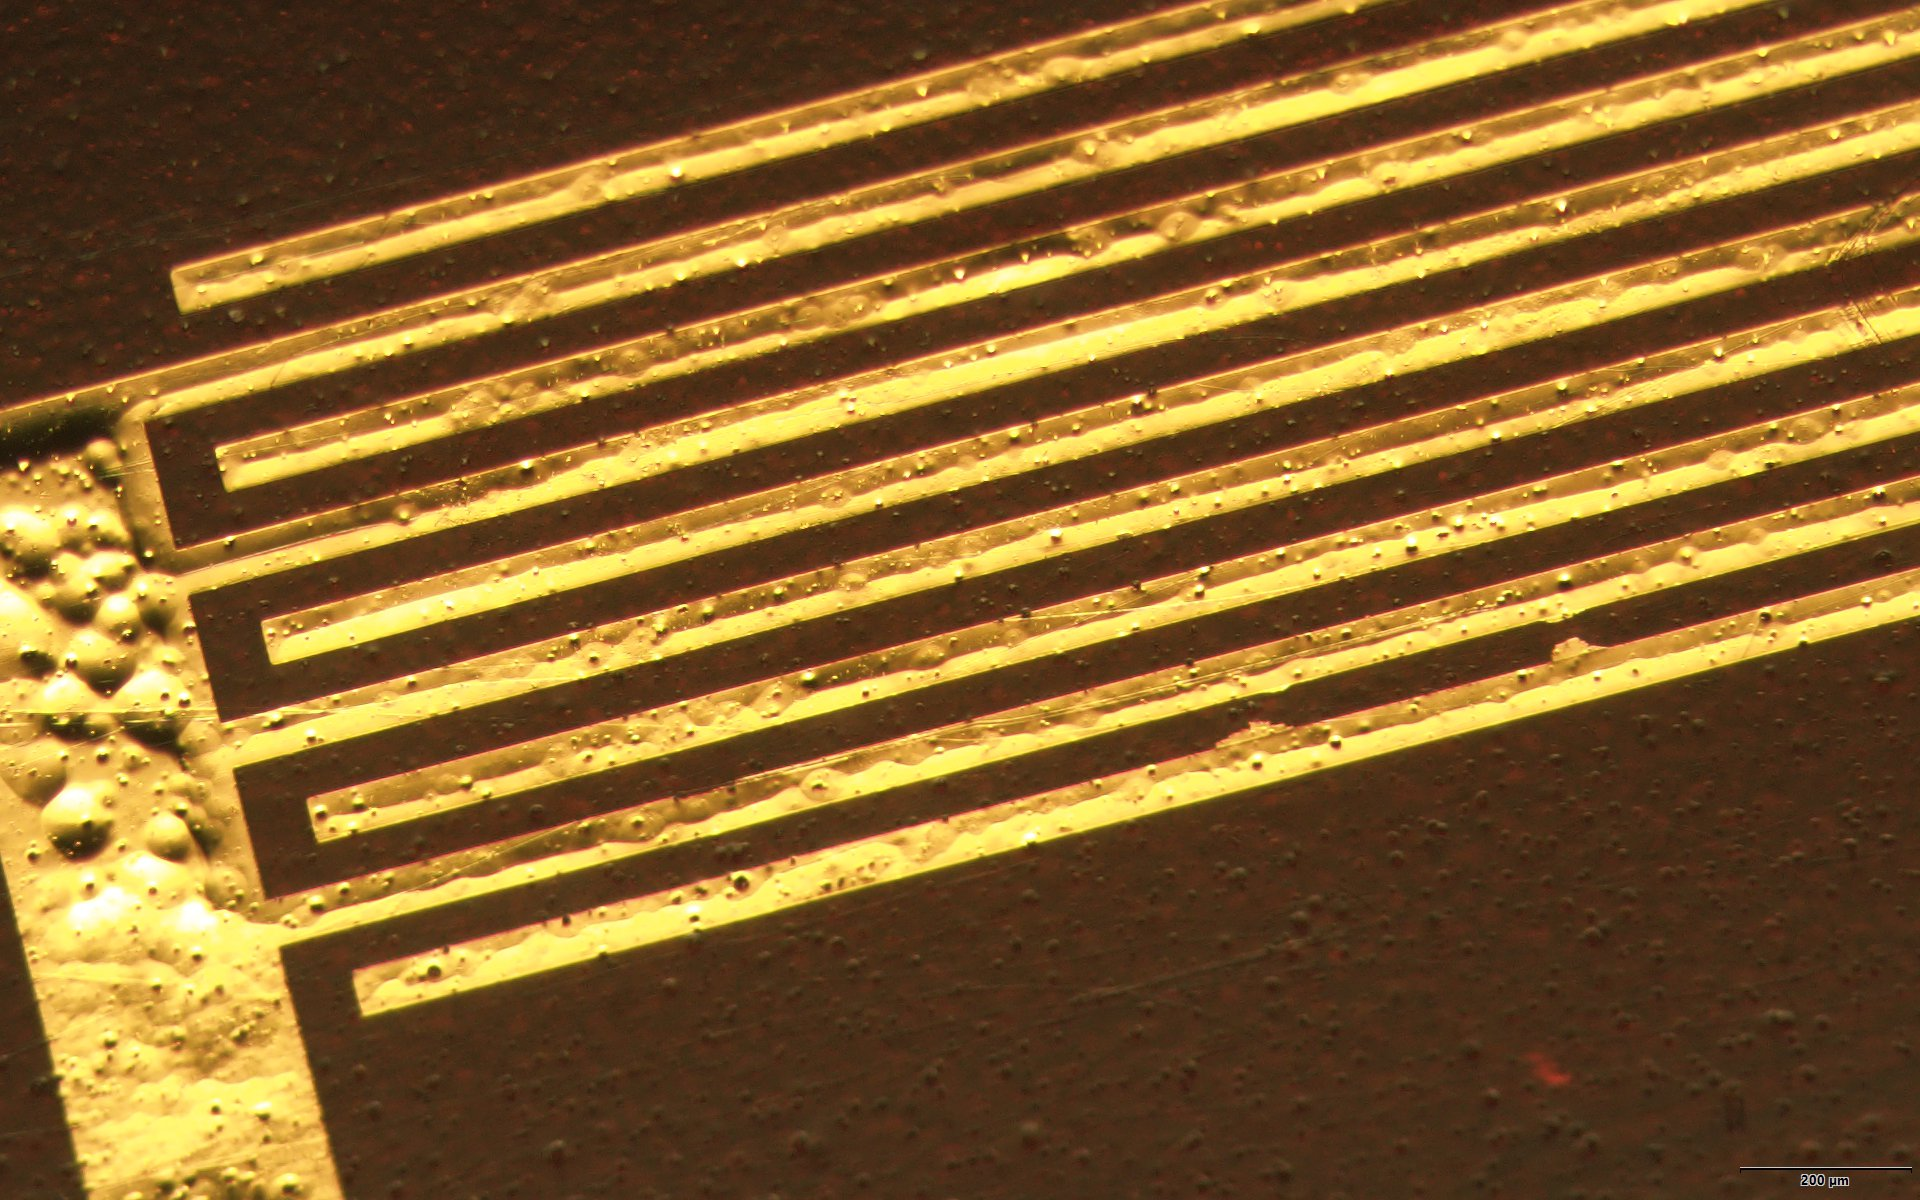
\includegraphics[width=0.4\textwidth]{../../data/photos/kapton/09072026_icn2/after/image_0722.jpg}
      \caption{Left: Gold residue in Source--Drain channel after lift-off process
               using single-layer S1813. Right: Clean channel after
               manual cotton-swab removal. This can lead to pattern damage.}
\end{figure}

\subsection{Proposed Solution}

A bilayer resist stack consisting of:
\begin{itemize}
    \item \textbf{PMGI SF5} (bottom layer): A polydimethylglutarimide-based
          lift-off resist that dissolves isotropically in alkaline developer,
          creating a controlled undercut beneath the imaging resist.
    \item \textbf{Shipley S1813} (top layer): The standard positive imaging
          resist, processed identically to the current protocol.
\end{itemize}

The bilayer stack is represented in Figure~\ref{fig:bilayer_diagram}.

\begin{figure}[hbt!]
      \centering
      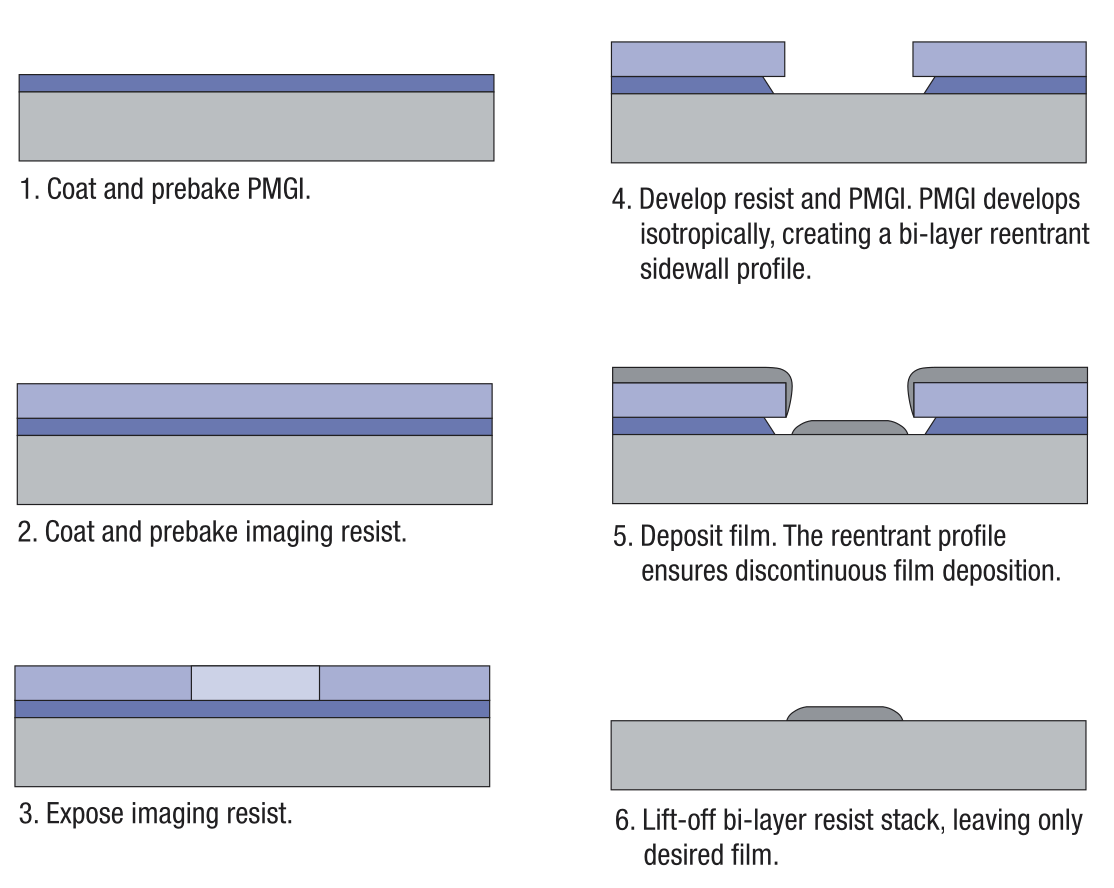
\includegraphics[width=0.5\textwidth]{bilayer-diagram.png}
      \caption{Schematic of the bilayer lift-off process.}
      \label{fig:bilayer_diagram}
\end{figure}

The undercut profile ensures that the evaporated metal film is
discontinuous at the resist edges, allowing the solvent to
penetrate and lift off the unwanted metal cleanly. DMSO at \SI{60}{\celsius}
replaces acetone/ultrasonic for a gentler, more effective strip.

\subsection{Required Materials}

\begin{table}[H]
\centering
\caption{Materials and chemicals required.}
\begin{tabular}{@{}lll@{}}
\toprule
\textbf{Material} & \textbf{Specification} & \textbf{Status} \\
\midrule
PMGI SF5 & MicroChem lift-off resist & In stock \\
Shipley S1813 & Positive photoresist & In stock \\
MF-319 & TMAH developer (2.2\%) & In stock \\
DMSO & Dimethyl sulfoxide, ULSI grade & Purchased \\
IPA & Isopropanol, cleanroom grade & In stock \\
DI water & \SI{18.2}{\mega\ohm\cdot\cm} & Available \\
Kapton HN & \SI{75}{\micro\m} polyimide foil & In stock \\
Si carrier wafer & 4-inch, for mounting & Available \\
\bottomrule
\end{tabular}
\end{table}

% ============================================================
\section{Process Overview}
% ============================================================

The bilayer lift-off process consists of eight major steps:

\begin{figure}[H]
\centering
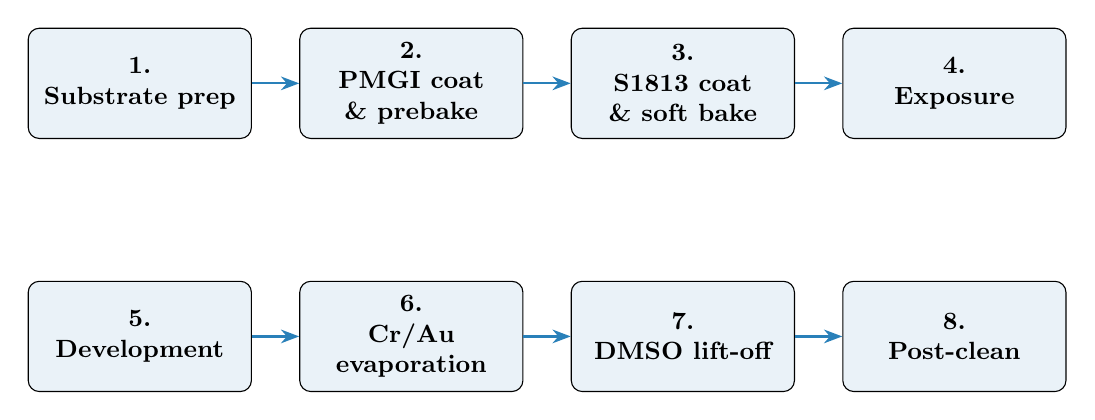
\begin{tikzpicture}[
    node distance=0.6cm,
    process/.style={draw, rounded corners=4pt, fill=stepcolor!10,
                    text width=2.6cm, minimum height=1.4cm,
                    align=center, font=\small\bfseries},
    arr/.style={-Stealth, thick, stepcolor}
]
% Top row
\node[process] (s1) {1.\\Substrate prep};
\node[process, right=of s1] (s2) {2.\\PMGI coat \& prebake};
\node[process, right=of s2] (s3) {3.\\S1813 coat \& soft bake};
\node[process, right=of s3] (s4) {4.\\Exposure};
% Bottom row
\node[process, below=1.8cm of s1] (s5) {5.\\Development};
\node[process, right=of s5] (s6) {6.\\Cr/Au evaporation};
\node[process, right=of s6] (s7) {7.\\DMSO lift-off};
\node[process, right=of s7] (s8) {8.\\Post-clean};
% Top row arrows
\foreach \i [evaluate=\i as \j using int(\i+1)] in {1,...,3}
    \draw[arr] (s\i.east) -- (s\j.west);
% Bottom row arrows
\foreach \i [evaluate=\i as \j using int(\i+1)] in {5,...,7}
    \draw[arr] (s\i.east) -- (s\j.west);
\end{tikzpicture}
\caption{Bilayer lift-off process overview.}
\label{fig:process_overview}
\end{figure}

% ============================================================
\section{Detailed Process Steps}
% ============================================================

% --- Step 1 ---
\subsection{Substrate Preparation and Mounting}

\begin{enumerate}[label=\alph*)]
    \item Cut Kapton foil to \SI{8}{\cm} $\times$ \SI{8}{\cm} pieces.
    \item Clean the Kapton substrate:
    \begin{enumerate}[label=\roman*)]
        \item Rinse with acetone
        \item Rinse with isopropanol
        \item Dry thoroughly with N$_2$ gun (front and back)
    \end{enumerate}
    \item Mount the Kapton on a clean Si carrier wafer using Kapton
          adhesive tape strips at the edges. Leave gaps between
          strips so air can escape during evaporation.
    \item Ensure both Kapton and carrier are \textbf{completely dry} ---
          trapped humidity at the interface ruins exposure and evaporation.
\end{enumerate}

\begin{warningbox}[Important]
Use \textbf{two different Si carriers}: one for photolithography
(coating + exposure + development) and a fresh one for evaporation.
This prevents adhesive residue from contaminating the evaporator.
\end{warningbox}

% --- Step 2 ---
\subsection{PMGI SF5 Coating and Prebake}

\begin{parambox}[PMGI SF5 Parameters]
\begin{tabular}{@{}ll@{}}
\toprule
\textbf{Parameter} & \textbf{Value} \\
\midrule
Spin speed & \SI{3000}{\rpm} \\
Spin time & \SI{45}{\second} \\
Acceleration & \SI{4000}{\rpm\per\second} \\
Expected thickness & \SIrange{0.5}{0.7}{\micro\m} \\
Prebake temperature & \SI{170}{\celsius} \\
Prebake time & \SI{5}{\min} \\
Bake mode & Contact hotplate \\
\bottomrule
\end{tabular}
\end{parambox}

\begin{enumerate}[label=\alph*)]
    \item Clean the spin coater chuck and support with acetone.
    \item Place a square of double-sided tape under the carrier wafer
          to prevent movement during spinning.
    \item Apply PMGI SF5 by pouring directly from the bottle (avoid pipette
          to prevent bubbles). Cover the wafer surface completely.
    \item Press START immediately after dispensing.
    \item Transfer to hotplate for prebake at \SI{170}{\celsius} for
          \SI{5}{\min}.
\end{enumerate}

\begin{tipbox}[Tip: Prebake Temperature]
The prebake temperature is the primary control for undercut rate.
At \SI{170}{\celsius} with MF-319, the undercut rate is approximately
\SI{33}{\angstrom\per\second} (\SI{0.33}{\nm\per\s}). This provides a
good balance between process control and development speed.

If undercut is too aggressive (features lifting off), increase prebake to
\SI{190}{\celsius} (\SI{28}{\angstrom\per\s}). If undercut is insufficient
(metal residue remains), decrease to \SI{150}{\celsius}
(\SI{42}{\angstrom\per\s}).
\end{tipbox}

% --- Step 3 ---
\subsection{S1813 Coating and Soft Bake}

\begin{parambox}[S1813 Parameters]
\begin{tabular}{@{}ll@{}}
\toprule
\textbf{Parameter} & \textbf{Value} \\
\midrule
Spin speed & \SI{5000}{\rpm} \\
Spin time & \SI{25}{\second} \\
Acceleration & \SI{4000}{\rpm\per\second} \\
Expected thickness & \SI{1.3}{\micro\m} \\
Soft bake temperature & \SI{75}{\celsius} \\
Soft bake time & \SI{1}{\min} \\
Bake mode & Contact hotplate \\
\bottomrule
\end{tabular}
\end{parambox}

\begin{enumerate}[label=\alph*)]
    \item Apply S1813 directly on top of the baked PMGI layer.
          \textbf{No intermixing occurs} --- PMGI is insoluble in the
          ethyl lactate solvent of S1813.
    \item Spin at \SI{5000}{\rpm} for \SI{25}{\s}.
    \item Soft bake at \SI{75}{\celsius} for \SI{1}{\min}.
\end{enumerate}

\begin{warningbox}[Do Not]
Do not press manually on the spinner lid during coating. Do not use
HMDS --- PMGI has excellent adhesion without primers.
\end{warningbox}

% --- Step 4 ---
\subsection{Exposure}

\begin{enumerate}[label=\alph*)]
    \item Expose the pattern using the Microwriter ML3 laser direct-write
          system.
    \item Use the \textbf{same dose} as the current S1813-only process.
    \item Recommended focus calibration: 9 points with offsets
          $(0,0)$, $(\pm30,0)$, $(0,\pm30)$, $(\pm20,\pm20)$\,\si{\micro\m}.
\end{enumerate}

% --- Step 5 ---
\subsection{Development (Single-Step Bilayer)}

\begin{parambox}[Development Parameters]
\begin{tabular}{@{}ll@{}}
\toprule
\textbf{Parameter} & \textbf{Value} \\
\midrule
Developer & MF-319 (TMAH 2.2\% with surfactant) \\
Mode & Immersion, manual stirring \\
Time & \SIrange{60}{90}{\second} \\
Rinse & DI water, $\geq$\SI{300}{\ml} \\
Dry & N$_2$ gun, front and back \\
\bottomrule
\end{tabular}
\end{parambox}

\begin{enumerate}[label=\alph*)]
    \item Carefully remove the Kapton foil from its Si carrier
          (do not bend).
    \item Immerse in MF-319 with the patterned face \textbf{up}.
    \item Stir manually for \SIrange{60}{90}{\second}.
    \item Rinse thoroughly with DI water (\SI{300}{\ml} or more).
    \item Dry \textbf{front and back} with N$_2$ gun --- residual water
          affects evaporation quality.
\end{enumerate}

\begin{tipbox}[Understanding the Development]
MF-319 develops \textbf{both layers simultaneously}:
\begin{itemize}
    \item The exposed S1813 dissolves in the developer (positive-tone
          behavior).
    \item The underlying PMGI dissolves \textbf{isotropically} ---
          sideways as well as downward --- creating the undercut.
\end{itemize}

The undercut depth is:
\begin{equation*}
    d_{\text{undercut}} = r_{\text{PMGI}} \times t_{\text{develop}}
\end{equation*}
where $r_{\text{PMGI}} \approx \SI{33}{\angstrom\per\s}$ at
\SI{170}{\celsius} prebake with MF-319.

For \SI{60}{\s}: $d \approx \SI{2.0}{\micro\m}$ of undercut. \\
For \SI{90}{\s}: $d \approx \SI{3.0}{\micro\m}$ of undercut.

Both values are sufficient for \SI{45}{\nm} of metal deposition.
\end{tipbox}

\begin{warningbox}[Critical]
Do \textbf{not} over-develop. Excessive undercut can cause small features
($<$\SI{10}{\micro\m}) to detach from the substrate. Start with
\SI{60}{\s} and increase only if metal residue persists after lift-off.
\end{warningbox}

% --- Step 6 ---
\subsection{Cr/Au Evaporation}

\begin{enumerate}[label=\alph*)]
    \item Re-mount the developed foil on a \textbf{fresh} Si carrier
          (different from the one used for photolithography).
    \item Provide the evaporator technician with the following parameters:
\end{enumerate}

\begin{parambox}[Evaporation Parameters --- Request to Technician]
\begin{tabular}{@{}ll@{}}
\toprule
\textbf{Parameter} & \textbf{Value} \\
\midrule
Adhesion layer & Cr, \SI{5}{\nm} \\
Electrode layer & Au, \SI{40}{\nm} \\
Cr deposition rate & $\leq$ \SI{0.2}{\angstrom\per\s} \\
Au deposition rate & $\leq$ \SI{0.5}{\angstrom\per\s} \\
Base pressure & $\leq$ \SI{5e-6}{\mbar} \\
Substrate rotation & None (incidence normal) \\
\bottomrule
\end{tabular}
\end{parambox}

\begin{tipbox}[Quality Check]
After evaporation, the Au film should appear \textbf{gold-colored and
reflective}. If it looks pinkish, opaque, or matte, inform the technician
--- this indicates oxidation or contamination and will cause poor SAM
formation and device performance.
\end{tipbox}

% --- Step 7 ---
\subsection{DMSO Lift-Off}

\begin{parambox}[DMSO Lift-Off Parameters]
\begin{tabular}{@{}ll@{}}
\toprule
\textbf{Parameter} & \textbf{Value} \\
\midrule
Solvent & DMSO (dimethyl sulfoxide), ULSI grade \\
Temperature & \SI{60}{\celsius} \\
Duration & \SIrange{2}{3}{\hour} \\
Ultrasonic & \textbf{None} (passive soak only) \\
Agitation & Gentle manual swirling every \SI{30}{\min} \\
\bottomrule
\end{tabular}
\end{parambox}

\begin{enumerate}[label=\alph*)]
    \item Place the sample in a glass beaker with fresh DMSO.
    \item Cover with a watch glass or petri dish (DMSO has low vapor
          pressure but should still be contained).
    \item Place on hotplate at \SI{60}{\celsius}.
    \item Soak for \SIrange{2}{4}{\hour}. Swirl gently every
          \SI{30}{\min}.
    \item The metal ``skin'' on top of the resist will begin to detach
          and float to the surface.
    \item Once lift-off is complete, remove sample and rinse immediately
          with IPA.
\end{enumerate}

\begin{warningbox}[Why DMSO, not Acetone?]
DMSO is preferred over acetone for the following reasons:
\begin{itemize}
    \item \textbf{No ultrasonic required}: The undercut profile allows
          DMSO to penetrate under the metal without mechanical agitation,
          preventing damage to delicate electrode patterns.
    \item \textbf{Better penetration}: DMSO has lower surface tension
          and higher boiling point than acetone, allowing it to wick into
          the undercut gap more effectively.
    \item \textbf{Non-toxic}: DMSO is not classified as toxic, unlike
          NMP (the traditional lift-off solvent).
    \item \textbf{Compatible with Kapton}: DMSO does not attack
          polyimide substrates.
\end{itemize}
\end{warningbox}

% --- Step 8 ---
\subsection{Post-Lift-Off Cleaning}

\begin{enumerate}[label=\alph*)]
    \item Rinse with IPA: 2 baths $\times$ \SI{15}{\min} each,
          fresh IPA per bath.
    \item Dry with N$_2$ gun.
    \item Inspect under microscope: verify clean channels with no
          residual gold.
\end{enumerate}

\begin{tipbox}[Expected Result]
After successful lift-off, gold should be present \textbf{only} in the
patterned electrode areas. The Source--Drain channels should be
\textbf{completely clean} --- no gold islands, no metal fences, no need
for cotton-swab removal. If residue persists, see
Section~\ref{sec:troubleshooting}.
\end{tipbox}

% ============================================================
\section{Troubleshooting}
\label{sec:troubleshooting}
% ============================================================

\begin{table}[H]
\centering
\caption{Common issues and solutions.}
\begin{tabular}{@{}p{4cm}p{4cm}p{5cm}@{}}
\toprule
\textbf{Symptom} & \textbf{Likely Cause} & \textbf{Solution} \\
\midrule
Gold residue in channels & Insufficient undercut & Increase develop time
    by \SI{15}{\s} increments. Check PMGI prebake temperature. \\
\midrule
Electrode pattern detaching & Excessive undercut & Decrease develop time
    or increase PMGI prebake temperature to \SI{190}{\celsius}. \\
\midrule
Lift-off takes $>$3\,h & DMSO too cold or undercut too small &
    Verify hotplate temperature. Increase develop time. \\
\midrule
Pinkish Au film & Evaporator contamination & Re-evaporate. Inform
    technician. \\
\midrule
Poor SAM formation & Au surface contaminated & Perform UV-ozone
    clean (\SI{25}{\min}) immediately before SAM. \\
\midrule
PMGI not adhering to Kapton & Surface contamination & Ensure dehydration
    bake at \SI{200}{\celsius}/\SI{5}{\min} before PMGI coating. \\
\bottomrule
\end{tabular}
\end{table}

% ============================================================
\section{Process Comparison}
% ============================================================

\begin{table}[H]
\centering
\caption{Comparison: Current protocol vs.\ Bilayer protocol.}
\begin{tabular}{@{}p{4cm}p{4.5cm}p{4.5cm}@{}}
\toprule
\textbf{Parameter} & \textbf{Current (S1813 only)} & \textbf{Bilayer
    (PMGI + S1813)} \\
\midrule
Photoresist layers & 1 (S1813) & 2 (PMGI SF5 + S1813) \\
Sidewall profile & Vertical & Undercut (re-entrant) \\
Lift-off solvent & Acetone + ultrasonido & DMSO at \SI{60}{\celsius} \\
Lift-off time & $3 \times \SI{15}{\min}$ + IPA baths &
    \SIrange{2}{3}{\hour} passive \\
Cotton swab needed & Yes (frequently) & \textbf{No} \\
Pattern damage risk & High & \textbf{Low} \\
Developer & MF-319 & MF-319 (same) \\
Exposure tool & Microwriter ML3 & Microwriter ML3 (same) \\
Additional equipment & None & Hotplate capable of \SI{170}{\celsius} \\
New chemicals & None & DMSO only \\
\bottomrule
\end{tabular}
\end{table}

% ============================================================
% References
% ============================================================

\bibliographystyle{ieeetr}
\nocite{*}
\bibliography{references}

\end{document}
